% Ch4: temporal compression of one trajectory.
% 101 simulation frames (t = 0..100) are padded to 105 = 8*13 + 1 by repeating
% the last frame (pad_frames_8n1). The causal LTX VAE encodes frame 0 alone into
% latent frame z_0 and each following group of 8 frames into one latent frame,
% giving 14 latent frames: z_0 (the DiT's clean condition) + z_1..z_13 (generated).
% The last group holds frames 97-100 plus the 4 padded copies.
\documentclass[tikz,border=4pt]{standalone}
\usepackage{amsmath,amssymb}
\usetikzlibrary{arrows.meta,calc,decorations.pathreplacing}
% Shared colours for the thesis TikZ figures. Same reference palette as
% scripts/thesis_figures.py (dataviz light mode), so diagrams and plots match.
\definecolor{ink}{HTML}{0B0B0B}
\definecolor{ink2}{HTML}{52514E}
\definecolor{muted}{HTML}{898781}
\definecolor{hair}{HTML}{C3C2B7}
\definecolor{neutralfill}{HTML}{F0EFEC}
\definecolor{blue}{HTML}{2A78D6}
\definecolor{bluefill}{HTML}{CDE2FB}
\definecolor{bluedark}{HTML}{184F95}
\definecolor{orange}{HTML}{EB6834}
\definecolor{orangefill}{HTML}{FBE0D3}
\definecolor{aqua}{HTML}{1BAF7A}
\definecolor{aquafill}{HTML}{D2F0E4}
\definecolor{violet}{HTML}{4A3AA7}
\definecolor{violetfill}{HTML}{E3E0F6}

% Trainable modules: orange fill + solid border. Frozen: neutral fill,
% dashed border, and every figure also labels the state in text.
\tikzset{
  every node/.style={font=\small, text=ink},
  box/.style={draw=hair, rounded corners=2pt, align=center, inner sep=4pt, line width=0.6pt},
  trainable/.style={box, fill=orangefill, draw=orange, line width=0.8pt},
  frozen/.style={box, fill=neutralfill, draw=muted, dashed},
  data/.style={box, fill=bluefill, draw=blue},
  latent/.style={box, fill=violetfill, draw=violet},
  cond/.style={box, fill=aquafill, draw=aqua},
  arr/.style={-{Stealth[length=5pt]}, draw=ink2, line width=0.7pt},
  note/.style={font=\footnotesize, text=ink2, align=center},
}


\begin{document}
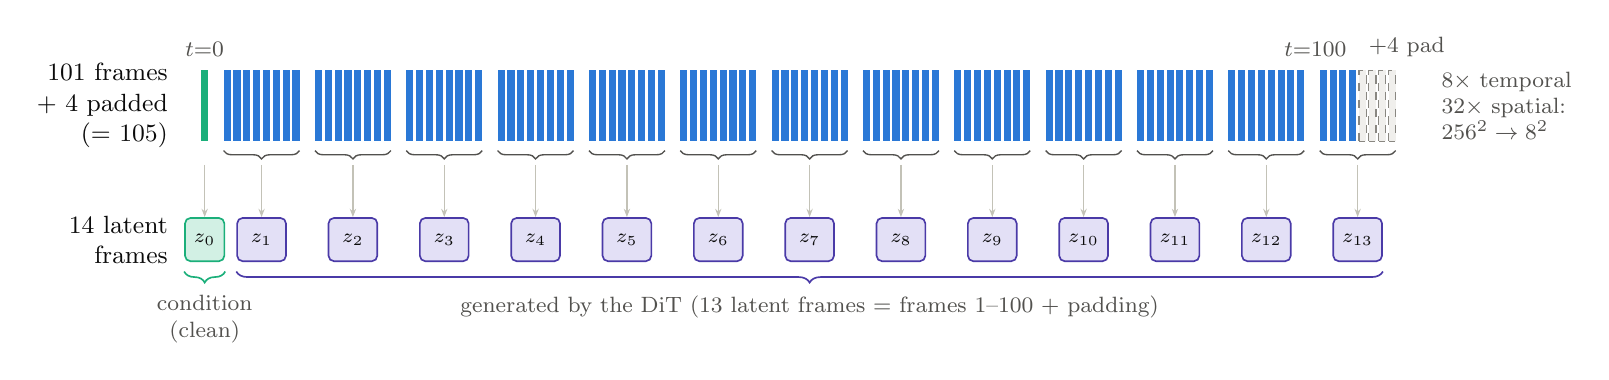
\begin{tikzpicture}
  \def\dx{0.125}   % horizontal pitch per frame
  \def\gap{0.16}   % extra space between 8-frame groups
  % x position of frame f: frame 0 alone, then groups of 8 separated by \gap
  \tikzset{declare function={fx(\f)=\f*\dx + (\f>0)*(floor((\f-1)/8)+1)*\gap;}}

  % frames
  \foreach \f in {0,...,104} {
    \pgfmathsetmacro{\x}{fx(\f)}
    \ifnum\f<101
      \ifnum\f=0
        \fill[aqua] (\x,0) rectangle ++(0.09,0.9);
      \else
        \fill[blue] (\x,0) rectangle ++(0.09,0.9);
      \fi
    \else
      \draw[muted, line width=0.4pt, dashed, fill=neutralfill] (\x,0) rectangle ++(0.09,0.9);
    \fi
  }
  \node[note, anchor=south] at ({fx(0)+0.045},0.95) {$t{=}0$};
  \node[note, anchor=south east] at ({fx(100)+0.09},0.95) {$t{=}100$};
  \node[note, anchor=south west] at ({fx(101)},0.95) {+4 pad};
  \node[anchor=east, align=right, font=\small] at (-0.3,0.45) {101 frames\\+ 4 padded\\(= 105)};

  % latents and grouping braces
  \foreach \g in {0,...,13} {
    \ifnum\g=0
      \pgfmathsetmacro{\xa}{fx(0)} \pgfmathsetmacro{\xb}{fx(0)+0.09}
    \else
      \pgfmathsetmacro{\xa}{fx(8*\g-7)} \pgfmathsetmacro{\xb}{fx(8*\g)+0.09}
    \fi
    \pgfmathsetmacro{\xm}{(\xa+\xb)/2}
    \ifnum\g>0
      \draw[decorate, decoration={brace, mirror, amplitude=3pt}, draw=ink2, line width=0.5pt] (\xa,-0.12) -- (\xb,-0.12);
    \fi
    \ifnum\g=0
      \node[cond, minimum width=0.5cm, minimum height=0.55cm, inner sep=1pt, font=\scriptsize] (z\g) at (\xm,-1.25) {$z_{0}$};
    \else
      \node[latent, minimum width=0.62cm, minimum height=0.55cm, inner sep=1pt, font=\scriptsize] (z\g) at (\xm,-1.25) {$z_{\g}$};
    \fi
    \draw[-{Stealth[length=3pt]}, draw=hair, line width=0.5pt] (\xm,-0.3) -- (z\g.north);
  }
  \node[anchor=east, align=right, font=\small] at (-0.3,-1.25) {14 latent\\frames};

  % annotations under the latents
  \draw[decorate, decoration={brace, mirror, amplitude=4pt}, draw=aqua, line width=0.6pt]
    ($(z0.south west)+(0,-0.12)$) -- ($(z0.south east)+(0,-0.12)$);
  \node[note, anchor=north, text=ink2] at ($(z0.south)+(0,-0.3)$) {condition\\(clean)};
  \draw[decorate, decoration={brace, mirror, amplitude=4pt}, draw=violet, line width=0.6pt]
    ($(z1.south west)+(0,-0.12)$) -- ($(z13.south east)+(0,-0.12)$);
  \node[note, anchor=north] at ($(z7.south)+(0,-0.3)$) {generated by the DiT (13 latent frames $=$ frames 1--100 + padding)};

  \node[note, anchor=west, align=left] at ({fx(104)+0.55},0.45) {8$\times$ temporal\\32$\times$ spatial:\\$256^2 \to 8^2$};
\end{tikzpicture}
\end{document}
